\documentclass[conference]{IEEEtran}
\IEEEoverridecommandlockouts
\usepackage{cite}
\usepackage{amsmath,amssymb,amsfonts}
\usepackage{graphicx}
\usepackage{booktabs}
\usepackage{multirow}
\usepackage{xcolor}
\usepackage{url}
\usepackage{tikz}
\usetikzlibrary{arrows.meta,positioning,calc}
\usepackage[hidelinks]{hyperref}

% Generated by python/scripts/export_paper_numbers.py -- do not edit by hand.
\newcommand{\mcN}{1000}
\newcommand{\mcFailUB}{0.38}
\newcommand{\mcHit}{99.96}
\newcommand{\mcHitLo}{99.91}
\newcommand{\mcHitHi}{99.99}
\newcommand{\mcMiss}{4}
\newcommand{\mcPulses}{9138}
\newcommand{\mcFh}{1.26}
\newcommand{\mcFhLo}{1.23}
\newcommand{\mcFhHi}{1.29}
\newcommand{\mcFhNinetyFive}{1.90}
\newcommand{\mcFhMax}{2.30}
\newcommand{\mcRms}{0.56}
\newcommand{\mcInR}{99.4}
\newcommand{\mcVpk}{589}
\newcommand{\mcRhoSlew}{0.94}
\newcommand{\mcRhoArms}{0.45}
\newcommand{\mcMissMed}{0.37}
\newcommand{\mcMissNinetyNine}{1.45}
\newcommand{\nBlackouts}{276}
\newcommand{\ezTrack}{1.01}
\newcommand{\ezCoast}{0.92}
\newcommand{\brier}{0.0045}
\newcommand{\tzFh}{1.65}
\newcommand{\tzHit}{99.90}
\newcommand{\abOtwoRms}{0.88}
\newcommand{\abOtwoMiss}{2$\to$77}
\newcommand{\abPtenFh}{0.42}
\newcommand{\abPthirtyRms}{-0.021}
\newcommand{\abPthirtyFh}{0.18}
\newcommand{\abAmbRms}{0.82}
\newcommand{\abOthreeRms}{-0.061}
\newcommand{\abOthreePrms}{4.8\times10^{-70}}
\newcommand{\stHit}{99.90}
\newcommand{\stMiss}{4}
\newcommand{\stFh}{1.01}
\newcommand{\stOthreeRms}{+0.002}
\newcommand{\stOthreePrms}{0.82}
\newcommand{\stDsixOthree}{0.17}
\newcommand{\stTwentyOthreeRms}{+0.021}
\newcommand{\stTwentyOthreeP}{1.1\times10^{-4}}
\newcommand{\stTwentyMiss}{14$\to$25}
\newcommand{\stPsureFh}{0.029}
\newcommand{\stPsureP}{3.1\times10^{-33}}
\newcommand{\stPsureMiss}{4$\to$4}
\newcommand{\scenarioRows}{%
A & 1.00 & 9/9 & 0.32\\
B & 1.00 & 9/9 & 0.53\\
C & 0.97 & 10/10 & 0.41\\
D1 & 0.71 & 10/10 & 0.40\\
D2 & 1.02 & 9/9 & 0.99\\
D3 & 1.27 & 9/9 & 0.32\\
D4 & 0.97 & 9/9 & 0.59\\
D5 & 1.16 & 9/9 & 0.69\\
D6 & 1.10 & 8/9 & 0.78\\}
\newcommand{\draftnote}{\\\textcolor{red}{PRELIMINARY DRAFT: numbers from the previous run (instant-fire threshold 0.999); final numbers pending}}


\newcommand{\D}{\mathcal{D}}
\newcommand{\Reng}{R_{\mathrm{eng}}}
\newtheorem{proposition}{Proposition}
\newtheorem{lemma}{Lemma}

\begin{document}

\title{Prediction-Matched Two-Degree-of-Freedom Fire Control of a Laser Turret against a Maneuvering Aerial Target}

\author{\IEEEauthorblockN{[Author Name]}
\IEEEauthorblockA{Department of Mechanical Engineering, Indian Institute of Technology Bombay\\
Code: {\footnotesize\url{https://github.com/VatshVan/Predictive-Tracking-and-Turret-Control-for-a-Maneuvering-Aerial-Target}}\draftnote}}

\maketitle

\begin{abstract}
We design the elevation-axis fire-control system of a pulsed-laser point-defence turret that must engage a maneuvering V-44 target from noisy 20\,Hz range/elevation radar, through radar blackouts of up to 0.5\,s. Because the laser is instantaneous, a hit needs the turret on the target's \emph{present} elevation, so the prescribed $t_p=0.5$\,s prediction must not lead the beam. We state precisely what the prediction is for. A jerk-model converted-measurement Kalman filter supplies the line-of-sight (LOS) angle and three derivatives. The third-order Taylor advance $A_3(s)$ forms the predicted reference, which carries the target's future motion into the controller. A two-input reference generator then removes the time advance exactly, $(\D+20)^3(y_d-\hat\theta)=0$, while an exact plant inverse uses the same derivatives to cancel the drive's lag. A PI loop ($68^\circ$ phase margin, 16\,dB gain margin) handles the rest. We prove that keeping the Taylor prediction inside the loop is possible only to order four, and show by test that doing so costs accuracy. A calibrated hit-probability rule decides when to fire. Over \mcN{} independent random engagements the design intercepted every target (failure probability $<\mcFailUB\%$, one-sided 97.5\% bound), with \mcHit\% of pulses hitting and a mean interception time of \mcFh\,s. It also intercepted all \hgN{} homotopy-guided adversarial engagements.
\end{abstract}

\begin{IEEEkeywords}
fire control, target tracking, Kalman filter, two-degree-of-freedom control, prediction, Monte Carlo validation
\end{IEEEkeywords}

% =====================================================================================
\section{Introduction}
Anti-aircraft predictors from the Kerrison predictor to the Bell Labs M9 aimed a gun at the target's future position, compensating projectile time of flight under a straight-flight assumption \cite{spec2026}. The Guardian problem differs in two ways. The weapon is a directed-energy laser with negligible propagation time, and the V-44 performs bounded maneuvers ($|\mathbf a|\le 20$\,m/s$^2$) and can vanish from radar for up to 0.5\,s \cite{spec2026}.

Three numbers make the problem hard. A 2\,m engagement radius is 1\,mrad at 2\,km, only $2.9\sigma_\theta$ of a single radar sample ($\sigma_\theta=0.35$\,mrad). An adversarial acceleration can displace the target by $\tfrac12 a_{\max}t_p^2=2.5$\,m in $t_p=0.5$\,s, more than the engagement radius. And the elevation drive has a lightly damped electromechanical mode at 8.9\,Hz ($\zeta=0.094$), so the reference must be smooth.

Target tracking for fire control is mature: Kalman target-state estimators \cite{barshalom2001}, the Singer and jerk maneuver models \cite{singer1970,mehrotra1997jerk,li2003survey}, converted-measurement filtering of polar radar data \cite{lerro1993}, and interacting multiple models \cite{mazor1998imm}. Homotopy classes of trajectories with consistent plan selection come from robot motion planning \cite{degroot2024tmpc}. Our contribution is not a new estimator but the way the blocks are \emph{matched} to this problem:
\begin{enumerate}
\item A precise account of the $t_p$ prediction: it supplies the future-motion information, and a two-input reference generator removes its time advance exactly. We prove that keeping the Taylor prediction inside the loop is possible only to order four, and test that alternative.
\item An estimator order chosen to match the plant: the drive has relative degree three, so its exact inverse needs the third LOS derivative, which a jerk-state filter provides.
\item A calibrated fire-now-or-wait rule over envelope-bounded maneuver classes.
\item Statistically validated design decisions: paired Monte Carlo ablations with multiplicity correction, stress-scenario noise ensembles, and homotopy-guided adversarial engagements that search the directions that defeat the controller rather than random ones.
\end{enumerate}

% =====================================================================================
\section{System Architecture and Design}
Fig.~\ref{fig:arch} shows the information flow. The radar returns $(r,\theta)$ every 50\,ms. The estimator converts each sample to Cartesian coordinates and updates a four-state-per-axis Kalman filter. Between samples, and during blackouts, it propagates the state with the motion model. From the nowcast $\hat{\mathbf x}(t)$ the predictor computes the LOS angle $\hat\theta$ and its derivatives and forms the predicted elevation reference $r(t)=\hat\theta(t+t_p)$. The reference generator turns $r$ into a smooth turret trajectory $y_d$ with its first three derivatives. These drive an exact plant-inverse feed-forward, and a feedback compensator $G_c(s)$ acts on $y_d-\theta$. The fire-control block compares the estimated target position with the measured turret angle and issues a pulse when the predicted hit probability justifies it. The voltage is limited to $\pm600$\,V, our assumed drive supply.\footnote{A 230\,V outlet, power-factor-corrected boost to a 700\,V DC link and an H-bridge; about 2.5\,kW peak, within a 16\,A socket \cite{mohan2003}. Details are in the repository.}

\begin{figure}[t]
\centering
\resizebox{\columnwidth}{!}{%
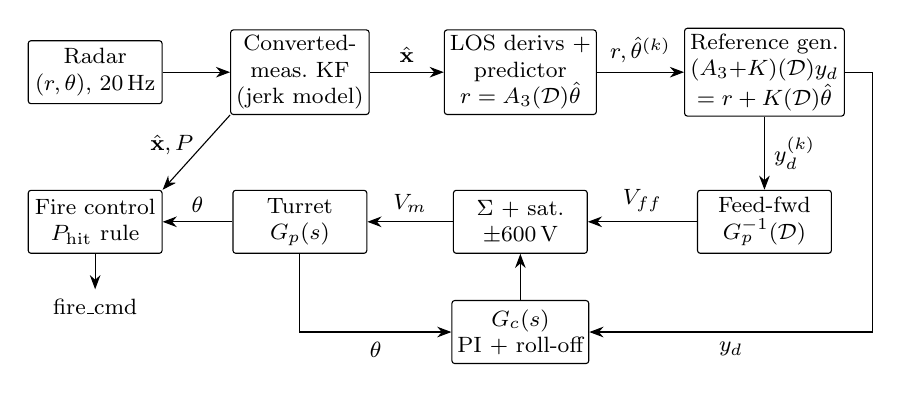
\begin{tikzpicture}[every node/.style={font=\footnotesize},
  blk/.style={draw, rounded corners=1pt, align=center, minimum height=8mm, minimum width=17mm, inner sep=2pt},
  >={Stealth[length=1.8mm]}]
\node[blk] (radar) at (0,0) {Radar\\$(r,\theta)$, 20\,Hz};
\node[blk] (kf) at (2.6,0) {Converted-\\meas.\ KF\\(jerk model)};
\node[blk] (pred) at (5.4,0) {LOS derivs +\\predictor\\$r=A_3(\D)\hat\theta$};
\node[blk] (ref) at (8.5,0) {Reference gen.\\$(A_3{+}K)(\D)y_d$\\$=r+K(\D)\hat\theta$};
\node[blk] (fire) at (0,-1.9) {Fire control\\$P_{\mathrm{hit}}$ rule};
\node[blk] (plant) at (2.6,-1.9) {Turret\\$G_p(s)$};
\node[blk] (sum) at (5.4,-1.9) {$\Sigma$ + sat.\\$\pm600$\,V};
\node[blk] (ff) at (8.5,-1.9) {Feed-fwd\\$G_p^{-1}(\D)$};
\node[blk] (gc) at (5.4,-3.3) {$G_c(s)$\\PI + roll-off};
\draw[->] (radar) -- (kf);
\draw[->] (kf) -- node[above]{$\hat{\mathbf x}$} (pred);
\draw[->] (pred) -- node[above]{$r,\hat\theta^{(k)}$} (ref);
\draw[->] (ref) -- node[right]{$y_d^{(k)}$} (ff);
\draw[->] (ff) -- node[above]{$V_{ff}$} (sum);
\draw[->] (sum) -- node[above]{$V_m$} (plant);
\draw[->] (ref.east) -- ++(0.35,0) |- node[pos=0.75,below]{$y_d$} (gc.east);
\draw[->] (plant.south) |- node[pos=0.75,below]{$\theta$} (gc.west);
\draw[->] (gc) -- (sum);
\draw[->] (kf.south west) -- node[left, pos=0.4]{$\hat{\mathbf x},P$} (fire.north east);
\draw[->] (plant) -- node[above]{$\theta$} (fire);
\draw[->] (fire.south) -- ++(0,-0.45) node[below]{fire\_cmd};
\end{tikzpicture}}
\caption{Predictive-feedback architecture. The reference generator receives the $t_p$ prediction $r$ and the nowcast $\hat\theta$; its output returns to $\hat\theta$, while the feed-forward uses the predicted motion.}
\label{fig:arch}
\end{figure}

% =====================================================================================
\section{Mathematical Modeling}

\subsection{Turret Elevation Plant}
Reflecting the motor through the $N=100$ gearbox gives $J_{eq}=J_t+N^2J_m=3200$\,kg\,m$^2$. Armature and turret-side torque balance give
\begin{equation}
L\dot i = V_m - Ri - NK_e\dot\theta,\qquad J_{eq}\ddot\theta = NK_ti - b\dot\theta,
\end{equation}
\begin{equation}
\begin{aligned}
G_p(s)=\frac{\theta}{V_m}&=\frac{NK_t}{s\,[(Ls+R)(J_{eq}s+b)+N^2K_tK_e]}\\
&=\frac{1000}{s(320s^2+3350s+1.0015{\times}10^6)}.
\end{aligned}
\label{eq:plant}
\end{equation}
The poles are $0$ and $-5.23\pm55.70j$\,rad/s (8.90\,Hz, $\zeta=0.094$). The large back-EMF term $N^2K_tK_e$ couples the electrical lag ($L/R=0.1$\,s) with a 3.2\,ms mechanical pole, which is what produces the resonance. The steady velocity gain is $1.0\times10^{-3}$\,rad\,s$^{-1}$/V, so tracking the largest LOS rate ($v_{\max}/r_{\min}=0.19$\,rad/s) needs about 190\,V. Forward-Euler integration of \eqref{eq:plant} is unstable for steps above 3.34\,ms, so all simulations integrate the plant at $\le1$\,ms.

\subsection{Radar Measurements}
With $\sigma_r=1$\,m and $\sigma_\theta=0.02^\circ$, the polar-to-Cartesian nonlinearity index $r\sigma_\theta^2/\sigma_r\approx2.4\times10^{-4}$ is negligible, so an EKF, a UKF and a converted-measurement filter are practically equivalent, and a particle filter is unjustified. We use the unbiased converted measurement $\mathbf z=\lambda^{-1}r[\cos\theta,\ \sin\theta]^\top$, $\lambda=e^{-\sigma_\theta^2/2}$, with its exact covariance \cite{mo1998unbiased}. This keeps the filter linear, so its steady-state behaviour can be analysed with the same LTI tools as the controller.

\subsection{Target Motion Model}
Each Cartesian axis carries position, velocity, acceleration and jerk, with jerk modeled as a first-order Gauss--Markov process \cite{mehrotra1997jerk}:
\begin{equation}
\dot{\mathbf s}=\begin{bmatrix}0&1&0&0\\0&0&1&0\\0&0&0&1\\0&0&0&-1/\tau_j\end{bmatrix}\mathbf s+\begin{bmatrix}0\\0\\0\\1\end{bmatrix}w,\quad E[w w']=\frac{2\sigma_j^2}{\tau_j}\delta,
\end{equation}
discretized exactly (Van Loan) for whatever interval elapses between calls. We use $\sigma_j=20$\,m/s$^3$ and $\tau_j=0.4$\,s. After every update the velocity and acceleration estimates are projected onto the admissible envelope ($|\mathbf v|\le157.5$, $|\mathbf a|\le23$; the specified bounds plus 5\% and 15\% margins), because the specification guarantees it. A $\chi^2$ innovation gate re-initialises the track after two consecutive implausible measurements, as would happen if the radar switched to another V-44 of a swarm.

\subsection{LOS Derivatives and Prediction}
Writing the target position as $z=x+jy$, the LOS angle is $\theta=\arg z$, so its derivatives follow from those of $\log z$. With $w_k=z^{(k)}/z$:
\begin{equation}
\dot\theta=\Im w_1,\quad \ddot\theta=\Im(w_2-w_1^2),\quad \dddot\theta=\Im(w_3-3w_1w_2+2w_1^3).
\end{equation}
These are exact for any trajectory, and are evaluated on the propagated nowcast. The predicted elevation reference is the Taylor advance
\begin{equation}
r(t)=A_3(\D)\hat\theta(t),\qquad A_3(s)=\sum_{k=0}^{3}\frac{(t_ps)^k}{k!},
\label{eq:pred}
\end{equation}
where $\D=d/dt$ and $t_p=0.5$\,s. This is the third-order truncation of $e^{st_p}$, the ideal time advance.

% =====================================================================================
\section{Controller Design and Analysis}

\subsection{Why Predict if the Laser Is Instantaneous?}
A hit is judged between the beam and the target's \emph{current} position, so the turret must satisfy $\theta(t)\approx\theta_T(t)$. Pointing the beam $t_p$ ahead would miss by about $r|\dot\theta|t_p$, i.e.\ 37\,m at 1.5\,km and 0.05\,rad/s, against $\Reng=2$\,m. The prediction is nevertheless essential, for three reasons.
\begin{enumerate}
\item \emph{Lag.} A loop that sees only the target's present angle trails it: a type-1 loop lags a ramp by $\dot\theta/K_v$. Removing that lag needs the target's future motion. The Taylor prediction \eqref{eq:pred} carries exactly that information, the velocity, acceleration and jerk terms of the error series. Requiring $1-T(s)A_3(s)=O(s^4)$ is the classical error-coefficient design ($K_v=1/t_p$ at first order).
\item \emph{Measurement loss.} During a blackout of up to 0.5\,s, the same length as $t_p$, the nowcast $\hat\theta(t)$ is itself a model prediction from the last radar update. Its quality decides whether the turret stays on target.
\item \emph{Firing.} Each pulse blocks the next for 1\,s, so the fire-now-or-wait decision needs where the target will be relative to the beam over the coming window (Section~\ref{sec:fire}).
\end{enumerate}

\subsection{Reference Generator: Using the Prediction's Information, Not Its Time Shift}
The generator takes both the prediction $r$ and the nowcast $\hat\theta$:
\begin{equation}
(A_3+K)(\D)\,y_d=r+K(\D)\hat\theta,\qquad A_3(s)+K(s)=\tfrac{t_p^3}{6}(s+p)^3 .
\label{eq:refgen}
\end{equation}
\begin{proposition}
With $r=A_3(\D)\hat\theta$, \eqref{eq:refgen} gives $(\D+p)^3(y_d-\hat\theta)=0$, so $y_d\to\hat\theta$ for any $t_p$.
\end{proposition}
The $t_p$ time advance is therefore removed exactly. What remains is the information: the generator outputs $y_d,\dots,\dddot y_d$, and $\dddot y_d$ inherits $\hat\theta'''$. The lag that the prediction exists to remove is instead cancelled by the exact plant inverse of Section~\ref{sec:ff}, which uses those derivatives, so $\theta=y_d\to\hat\theta$: the turret sits on the present estimate without lag. The deviation from the nowcast, caused only by each estimator correction, decays with a triple pole at $-p$ ($p=20$\,rad/s, $K(s)=165.7+24.5s+1.125s^2$).

\emph{Keeping the prediction in the loop.} The alternative is $T=1/A_n$, so $T(s)A_n(s)=1$ exactly; its deviation poles are then the roots of $A_n$.
\begin{lemma}
The Taylor sections $A_n(s)=\sum_{k\le n}(t_ps)^k/k!$ are Hurwitz for $n\le4$ and unstable for $n\ge5$. Their least-damped root has $\zeta=1, 0.71, 0.36, 0.11$ for $n=1,\dots,4$.
\end{lemma}
More generally, a stable reference polynomial can match $e^{st_p}$ to order 4, or to order 5 with two extra free coefficients ($\zeta\le0.14$), and no further in practice. Keeping the velocity term exact ($p_1=t_p$) forces $\sum1/s_i=-t_p$, so a cubic's slowest pole decays no faster than $3/t_p=6$\,rad/s. Order four is therefore the hard ceiling on a loop that keeps the prediction, and it comes with slow, poorly damped poles: $A_3$ has roots $-1.40\pm3.61j$ and $-3.19$, and in our first prototype a 0.4\,rad slew overshot by 46\,m. Section~\ref{sec:inloop} tests this alternative against \eqref{eq:refgen}. We realise \eqref{eq:refgen} as a cascade with gains $(p/3,\,p,\,3p)$ whose intermediate rate and acceleration demands are saturated at 0.58\,rad/s and 2.5\,rad/s$^2$. In the small-deviation regime this is exactly linear, and during large acquisition slews it respects the voltage and current limits without the chatter that state clamping produced in our trials.

\subsection{Feed-Forward and Feedback}
\label{sec:ff}
The reference generator supplies $y_d,\dot y_d,\ddot y_d,\dddot y_d$ without numerical differentiation. The plant has relative degree three, so its exact inverse
\begin{equation}
V_{ff}=G_p^{-1}(\D)y_d=0.32\,\dddot y_d+3.35\,\ddot y_d+1001.5\,\dot y_d
\end{equation}
is realisable. This is the second reason for a jerk-state estimator: $\dddot y_d$ inherits $\hat\theta'''$. With an exact model, $\theta=y_d$ and the feedback acts only on initial conditions, sampling (ZOH) error and model mismatch. We use
\begin{equation}
G_c(s)=K_p\Big(1+\frac{1}{T_is}\Big)\frac{1}{\tau_fs+1},
\end{equation}
with $K_p=4000$\,V/rad, $T_i=1$\,s and $\tau_f=0.03$\,s, giving a crossover at 4.1\,rad/s, a decade below the resonance. The resonance stays 16\,dB below unity loop gain, so it is gain-stabilised without a notch. Table~\ref{tab:margins} gives margins of the implemented discrete compensator (backward-Euler integral, exact first-order filter) with a ZOH plant. They barely change down to the 20\,Hz radar rate. Conditional integration prevents windup at the $\pm600$\,V limit.

\begin{table}[t]
\centering
\caption{Loop margins of the implemented $G_c$ with ZOH plant}
\label{tab:margins}
\begin{tabular}{lccc}
\toprule
Sampling & $\omega_c$ [rad/s] & PM [deg] & GM [dB] \\
\midrule
continuous & 4.10 & 68.5 & 16.1\\
100\,Hz & 4.12 & 68.5 & 16.1\\
20\,Hz & 4.19 & 67.4 & 18.6\\
\bottomrule
\end{tabular}
\end{table}

\subsection{Noise, Prediction Error and Measurement Loss}
Because $y_d\to\hat\theta$ exactly, the transfer from radar noise to turret angle is the estimator's own, and loop bandwidth does not trade against noise. The deviation pole $p$ sets how fast each measurement correction is absorbed. Low $p$ lags maneuvers, high $p$ slows acquisition (Section~\ref{sec:ablation}). During a blackout the filter coasts. Its covariance grows like the jerk-model integral, and the worst-case drift is bounded by $\tfrac12a_{\max}t^2$ (2.5\,m at 0.5\,s), so no controller can guarantee a hit late in a long blackout. On recovery the first measurement collapses the covariance, and the reference generator absorbs the correction at $p=20$\,rad/s, without a step into the lightly damped drive.

\subsection{Fire Control}
\label{sec:fire}
For the estimated target and the measured turret angle, the signed beam-to-target cross-range offset $d$ is Gaussian with the filter's cross-range standard deviation $\sigma$. To hedge unmodeled maneuvers since the last radar sample (age $\tau$), we evaluate it for 17 maneuver classes: the nominal estimate plus constant accelerations of magnitude $a_{\max}/2$ and $a_{\max}$ in eight directions, each displaced by $\tfrac12(\mathbf a_i-\hat{\mathbf a})\tau^2$. The hit probability is the mixture
\begin{equation}
P_{\mathrm{hit}}=\sum_i w_i\Big[\Phi\Big(\tfrac{\Reng-d_i}{\sigma}\Big)-\Phi\Big(\tfrac{-\Reng-d_i}{\sigma}\Big)\Big],
\end{equation}
with weight 0.5 on the nominal class. A pulse also requires at least 80\% of classes inside $\Reng$ and at least 8 radar updates. Each pulse blocks the next for 1\,s, so firing is a fire-now-or-wait decision:
\begin{itemize}
\item \emph{Tracking:} fire at once if $P_{\mathrm{hit}}\ge0.99$. Otherwise arm at $0.90$ and fire when $P_{\mathrm{hit}}$ has peaked (fallen by 0.02) or after 0.3\,s.
\item \emph{Coasting:} certainty can only decay, so fire only while $P_{\mathrm{hit}}\ge0.95$, which in practice means early in a loss.
\end{itemize}

% =====================================================================================
\section{Simulation and Results}
\label{sec:results}

\subsection{Protocol}
The simulator follows the evaluation interface. At each controller step it calls the generator, then the controller, and judges a pulse on every $0\to1$ edge of \texttt{fire\_cmd} that is at least 1\,s after the last pulse: a hit if the target lies within 2\,m of the beam ray. It then integrates the plant with RK4 at 1\,ms under a zero-order-hold voltage, with mechanical stops. The controller runs at 100\,Hz unless stated and reads its own time step from $t$. The turret starts at rest at $0^\circ$. The Python implementation and the submitted MATLAB \texttt{turret\_controller.m} agree to $3\times10^{-9}$\,V with identical fire commands on 12 replayed runs.

Beyond scenarios A--C we built six stress scenarios modelling plausible hidden cases: D1, a pull-up that starts \emph{inside} a late blackout; D2, a near-$a_{\max}$ weave; D3, a close pass to 853\,m approaching $+85^\circ$; D4, four blackouts; D5, weave plus blackout at short range; and D6, $\pm18$\,m/s$^2$ reversals with 450\,m/s$^3$ jerk. The Monte Carlo generator draws an initial range $U(1500,2000)$\,m, elevation $U(8^\circ,55^\circ)$ and speed $U(70,150)$\,m/s, an inbound heading $\pm40^\circ$, a sum of three random sinusoids per axis plus an optional break maneuver scaled to a peak of $U(0.4,1)\,a_{\max}$, and one or two blackouts with onset $\ge1$\,s and duration $\le0.5$\,s. Inadmissible draws are rejected. The repository's detailed experimental report (\texttt{docs/report}) documents every scenario, figure and statistical test summarised below.

\subsection{Standardized and Stress Scenarios}
Table~\ref{tab:scen} lists single runs, and Fig.~\ref{fig:scenC} shows Scenario C. The turret slews at the 0.58\,rad/s limit, arrives within about 1\,s, and fires immediately. During the blackout $P_{\mathrm{hit}}$ decays honestly and no pulse is wasted. After recovery the error returns inside 1\,m. Across the 450-run noise ensemble of all nine scenarios (50 noise realisations each), every engagement was intercepted and \stHit\% of pulses hit (\stMiss{} misses), with a mean first hit of \stFh\,s.

\begin{table}[t]
\centering
\caption{Scenario results (single realisation, 1\,kHz controller)}
\label{tab:scen}
\begin{tabular}{lccc}
\toprule
Scenario & First hit [s] & Pulses hit & Pointing RMS [m]\\
\midrule
\scenarioRows
\bottomrule
\end{tabular}
\end{table}

\begin{figure}[t]
\centering
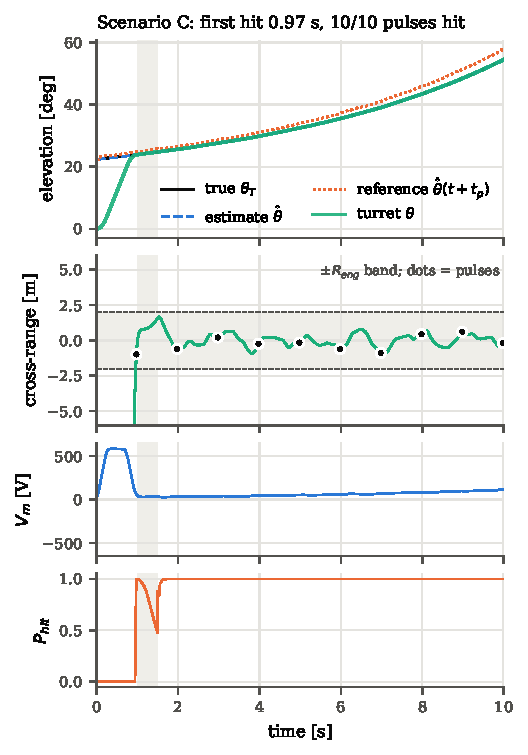
\includegraphics[width=\columnwidth]{figures/scenario_C.pdf}
\caption{Scenario C (blackout shaded). Top: true, estimated and predicted ($t_p$-ahead) elevation and the turret. Second: cross-range pointing error with $\pm\Reng$ band and pulses. Bottom: motor voltage and $P_{\mathrm{hit}}$.}
\label{fig:scenC}
\end{figure}

\begin{figure*}[t]
\centering
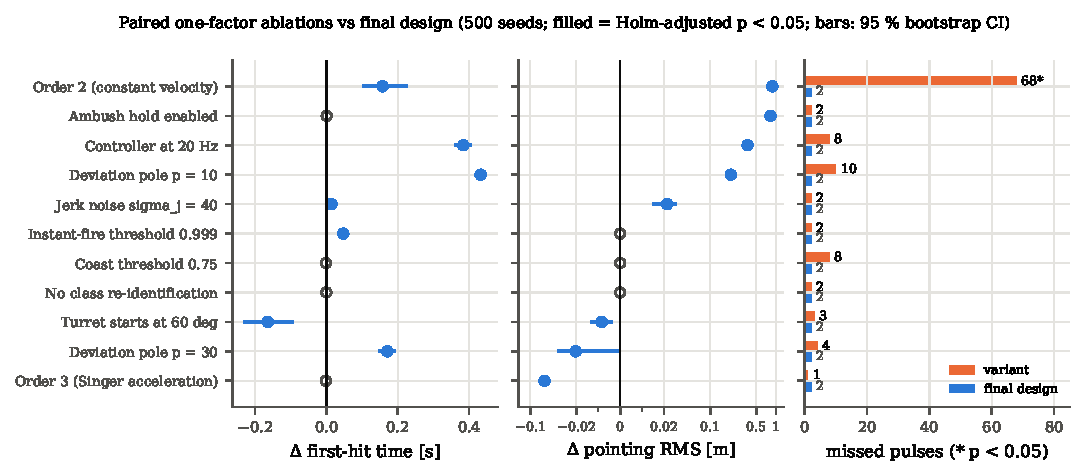
\includegraphics[width=0.85\textwidth]{figures/mc_ablation_forest.pdf}
\caption{Paired one-factor ablations against the final design (500 seeds). Points: mean paired difference with 95\% bootstrap CI; filled when the Holm-adjusted $p<0.05$. Right: missed pulses.}
\label{fig:forest}
\end{figure*}

\subsection{Monte Carlo Performance}
Over \mcN{} random engagements the design intercepted every target. The Wilson 95\% upper bound on the failure probability is \mcFailUB\% \cite{wilson1927}. \mcHit\% of \mcPulses{} pulses hit; the cluster-bootstrap 95\% CI is [\mcHitLo, \mcHitHi]\%, resampling whole engagements because pulses within one are correlated \cite{efron1993}. The median pulse miss distance was \mcMissMed\,m, and the 99th percentile \mcMissNinetyNine\,m. Interception took \mcFh\,s on average (CI [\mcFhLo, \mcFhHi]\,s; 95th percentile \mcFhNinetyFive\,s; maximum \mcFhMax\,s). It is acquisition-limited: the first-hit time correlates with the initial slew angle at Spearman $\rho=\mcRhoSlew$ (Fig.~\ref{fig:mc}), and not with maneuver intensity. Pointing accuracy, by contrast, degrades gracefully with maneuver intensity ($\rho=\mcRhoArms$ with RMS target acceleration; median RMS \mcRms\,m; \mcInR\% of the time within $\Reng$). After acquisition, the median pointing error settles near 0.35\,m and the 90th percentile stays below 1\,m over 300 logged engagements. That is the size of the estimation error itself, as $y_d\to\hat\theta$ predicts. Peak voltage was \mcVpk\,V.

Fig.~\ref{fig:blackout} aligns \nBlackouts{} blackouts. Pointing error peaks at a median of about 0.8\,m about 0.35\,s after onset and recovers within about 0.4\,s. Two checks show the probabilities behind the firing rule are honest. The normalised estimation error has $E[z^2]=\ezTrack$ while tracking (ideal 1) and \ezCoast{} while coasting, and the observed hit frequency follows the predicted $P_{\mathrm{hit}}$ (Brier score \brier{} over about 270\,000 controller samples), conservatively in mid-range bins.

\begin{figure*}[t]
\centering
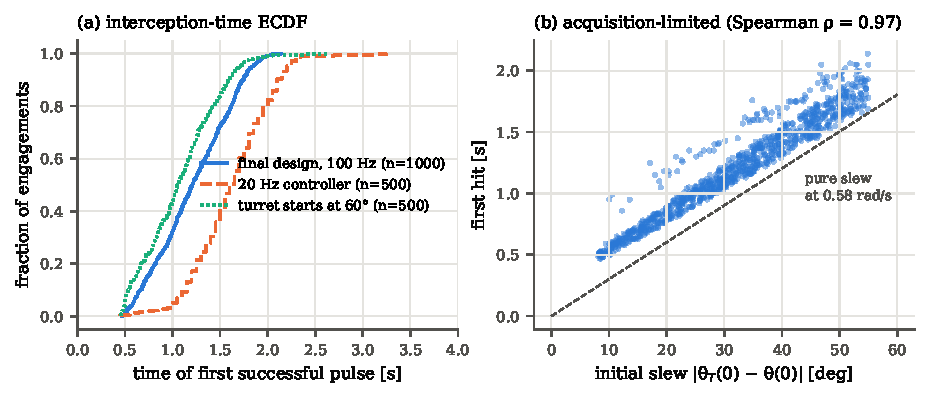
\includegraphics[width=0.7\textwidth]{figures/mc_first_hit.pdf}
\caption{Interception time over the Monte Carlo campaign. (a) ECDFs for the final design, a 20\,Hz controller and a turret starting at $60^\circ$. (b) First-hit time against the initial slew angle; the dashed line is a pure slew at the 0.58\,rad/s limit.}
\label{fig:mc}
\end{figure*}

\begin{figure}[t]
\centering
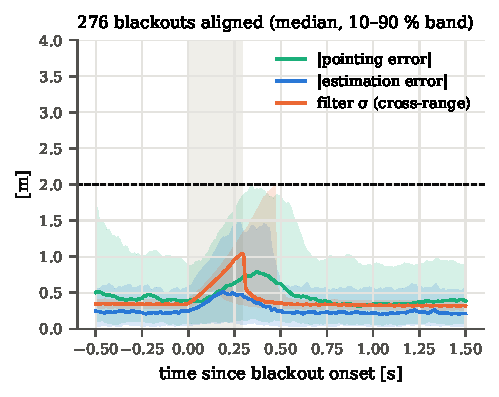
\includegraphics[width=0.92\columnwidth]{figures/mc_blackout_aligned.pdf}
\caption{Pointing error, estimation error and filter standard deviation aligned on blackout onset (median and 10--90\% band; median blackout duration shaded).}
\label{fig:blackout}
\end{figure}

\subsection{Design Decisions under Paired Statistics}
\label{sec:ablation}
Each design choice was tested as a one-factor change on the same 500 seeds as the final design, so trajectory, blackouts and noise are paired. We used Wilcoxon signed-rank tests for timing and pointing \cite{wilcoxon1945}, a sign-flip permutation test for missed pulses, and Holm correction over the 11 comparisons \cite{holm1979}. The results (Fig.~\ref{fig:forest}):
\begin{itemize}
\item A constant-velocity filter (order 2) is decisively worse: pointing RMS $+\abOtwoRms$\,m, missed pulses \abOtwoMiss, and \abOtwoLost{} interceptions lost.
\item A slower deviation pole ($p=10$) delays interception by \abPtenFh\,s. A faster one ($p=30$) gains only $\abPthirtyRms$\,m RMS but delays interception by \abPthirtyFh\,s.
\item The ambush hold from our early design (park the beam where every maneuver class must cross) worsens pointing by \abAmbRms\,m without gaining hits, so it was rejected.
\item Class re-identification at blackout recovery had no measurable effect (misses \noreidMiss{} over 1\,000 seeds); the Kalman update with the coasted covariance already does that job.
\end{itemize}

Estimator order needs both test sets:
\begin{itemize}
\item On the smooth random maneuvers, order 3 (Singer acceleration) points slightly better ($\abOthreeRms$\,m, $p=\abOthreePrms$).
\item On the stress ensembles the two orders tie overall at 100\,Hz ($\stOthreeRms$\,m, $p=\stOthreePrms$). Order 4 is better on the high-jerk scenario D6 (order 3: $+\stDsixOthree$\,m).
\item At a 20\,Hz controller, order 4 is better overall ($\stTwentyOthreeRms$\,m for order 3, $p=\stTwentyOthreeP$; misses \stTwentyMiss).
\end{itemize}
Since a hidden case is likelier to be jerky than smooth, we keep order 4. We also tested a stricter instant-fire threshold of 0.999. It delayed interception by \stPsureFh\,s ($p=\stPsureP$) with no change in misses (\stPsureMiss), so the final design uses 0.99.



\subsection{Prediction in the Loop, and Homotopy-Guided Adversaries}
\label{sec:inloop}
\emph{Adversary.} Random maneuvers rarely probe the controller's weak directions, so we also generated engagements by homotopy class, following \cite{degroot2024tmpc}. In the plane of time and the target's signed cross-range offset from the beam, the obstacles are the firing events $\{t_k\}\times[-\Reng,\Reng]$. A target path's class is the side on which it passes each event (above, through, below). For each of \hgN{} base engagements we find the frozen design's firing times, then reverse the target's normal acceleration at $a_{\max}$ (finite jerk) just before each shot toward the side its class requires (above, below, crossing either way, alternating). The lead time is chosen to maximise the miss, and the envelope is enforced. The misses do follow the attacked side. The adversary is still weak: 63\% of cases left every pulse hitting.

\emph{Results.} Table~\ref{tab:inloop} compares reference laws that keep the Taylor prediction in the loop with \eqref{eq:refgen}. Every design intercepted all random and all adversarial engagements. Keeping the prediction costs 0.4--4.4\,m of pointing accuracy on random engagements and more misses there. Under attack its slow poles miss less per pulse, because the 20\,rad/s design follows each estimator correction. But the slow designs are on target less of the time and shoot less, so \eqref{eq:refgen} still delivers the most hits. It also does so when the adversary is re-tuned against each alternative. A homotopy-class fire planner with the plan-consistency rule of \cite{degroot2024tmpc} did not change misses significantly (\homMiss{} random, \homHgMiss{} adversarial), so the mixture rule stays.

\begin{table}[t]
\centering
\caption{Reference laws on \mcN{} random (MC) and \hgN{} adversarial (HG) engagements}
\label{tab:inloop}
\setlength{\tabcolsep}{3.5pt}
\begin{tabular}{lcccc}
\toprule
& \multicolumn{2}{c}{MC} & \multicolumn{2}{c}{HG}\\
\cmidrule(lr){2-3}\cmidrule(l){4-5}
Reference law & RMS [m] & misses & miss [\%] & hits\\
\midrule
\researchRows
\bottomrule
\end{tabular}
\end{table}

\subsection{Controller Rate}
Run on 24 cases per rate from 20\,Hz to 5\,kHz, the controller intercepted every target. Performance saturates near 200\,Hz. At 20\,Hz the mean first hit rises to \tzFh\,s, with \tzHit\% of pulses hitting over 500 Monte Carlo runs. The MATLAB controller costs 0.51\,ms per call, so we recommend 100\,Hz--1\,kHz and a plant step of $\le1$\,ms.

% =====================================================================================
\section{Final Evaluation}
\label{sec:final}
The evaluation cases are hidden; expectations for them rest on three lines of evidence.
\begin{itemize}
\item \emph{Interception.} All \mcN{} independent random engagements were intercepted, bounding the failure probability below \mcFailUB\% (one-sided 97.5\%, Wilson). Runs that reuse those seeds (20\,Hz, $60^\circ$ start) or replicate the stress scenarios with new noise (\otherN{} in all) are not pooled into the bound; all were intercepted, as were the \hgN{} adversarial engagements and \pertOK{} engagements with $R$, $L$, $J_{eq}$ and $b$ each perturbed within $\pm20\%$ (\pertMiss{} misses in \pertPulses{} pulses).
\item \emph{Interception time is predictable from geometry.} A fit gives $t_{\mathrm{hit}}\approx\slewA+\slewB\,\Delta\theta_0$\,s, with $\Delta\theta_0$ the initial slew in degrees ($R^2=\slewR$, $\pm\slewPI$\,s at 95\%). The slope matches the 0.58\,rad/s slew limit, and the worst admissible slew ($95^\circ$) predicts \slewWorst\,s.
\item \emph{Independence from the evaluation script.} We tried \ifVariants{} plausible calling conventions: held or stale measurements re-asserted as valid, irregular radar timing at steps that do not divide 50\,ms, random initial turret angles, forward-Euler plant integration, and 1\,kHz calls. All \ifOK{} of \ifN{} engagements were intercepted, with at least \ifHitMin\% of pulses hitting.
\end{itemize}
The evidence does not extend to jerk beyond about 450\,m/s$^3$, blackouts longer than 0.5\,s, or plant errors beyond $\pm20\%$; for the last, robustness rests on the margins of Table~\ref{tab:margins}.

% =====================================================================================
\section{Conclusions}
An instantaneous laser must point at the target's present position, so the prescribed $t_p$ prediction cannot lead the beam. Its value is the future-motion information it carries: a two-input reference generator removes its time advance exactly, and the jerk-state estimate feeds the plant inverse that removes the turret's lag. Keeping the Taylor prediction inside the loop is bounded at fourth order, forces slow poles, and costs accuracy and hits. The frozen design intercepted every random, adversarial and plant-perturbed engagement we tested. Its limits: interception time is set by slew kinematics, late blackout shots cannot be guaranteed, and shot-timed maneuvers raise the per-pulse miss rate to \hgMissRate\%, though no engagement was lost.

\bibliographystyle{IEEEtran}
\bibliography{refs}

\end{document}
